\documentclass[crop, tikz]{standalone}
\usepackage{tikz}
\usepackage{amsmath}

\usetikzlibrary{decorations.pathmorphing, positioning}

\definecolor{echoreg}{HTML}{2cb1e1}
\definecolor{echodrk}{HTML}{0099cc}

\tikzstyle{mybox} = [text=black, very thick,
    rectangle, rounded corners, inner sep=10pt, inner ysep=20pt]
\tikzstyle{fancytitle} =[text=black]

\newcommand{\yslant}{0.5}
\newcommand{\xslant}{-0.6}

\newcommand\overmat[3]{%
  \makebox[0pt][l]{$\smash{\color{#3}\overbrace{\phantom{%
    \begin{matrix}#2\end{matrix}}}^{\text{#1}}}$}#2}
\newcommand\undermat[3]{%
  \makebox[0pt][l]{$\smash{\color{#3}\underbrace{\phantom{%
    \begin{matrix}#2\end{matrix}}}_{\text{#1}}}$}#2}
\newcommand\partialphantom{\vphantom{\frac{\partial e_{P,M}}{\partial w_{1,1}}}}

\begin{document}
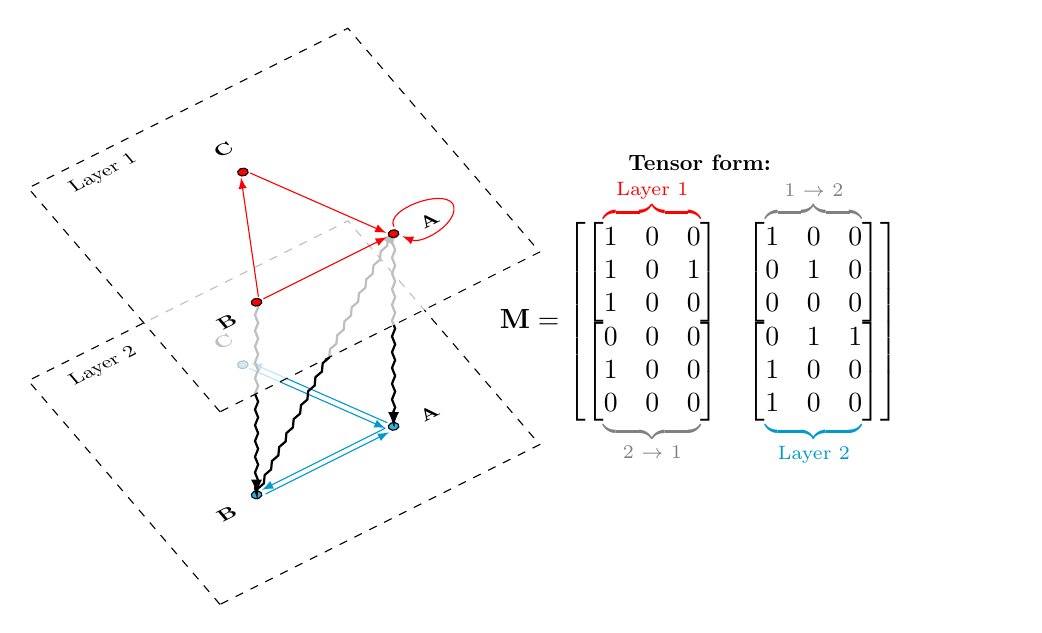
\begin{tikzpicture}[scale=0.58,every node/.style={minimum size=1cm},on grid]

	\node [mybox, scale=1.0] at (10.5, 2) (box){%
		\begin{minipage}{0.6\textwidth}
			\[  {\mathbf M} = {\left[
			\begin{matrix}
				\left[\overmat{\textcolor{red}Layer 1}{
				\begin{matrix}
					1 & 0 & 0\\
					1 & 0 & 1\\
					1 & 0 & 0\\
				\end{matrix}}{red}\right] & \left[\overmat{1 $\rightarrow$ 2}{
				\begin{matrix}
					1 & 0 & 0\\
					0 & 1 & 0\\
					0 & 0 & 0\\
				\end{matrix}}{gray}\right]\\
				\left[\undermat{2 $\rightarrow$ 1}{
				\begin{matrix}
					0 & 0 & 0\\
					1 & 0 & 0\\
					0 & 0 & 0\\
				\end{matrix}}{gray}\right] & \left[\undermat{\textcolor{echodrk}Layer 2}{
				\begin{matrix}
					0 & 1 & 1\\
					1 & 0 & 0\\
					1 & 0 & 0\\
        		\end{matrix}}{echodrk}\right]\\	
			\end{matrix}\right]}\]
    	\end{minipage}
	};
	
	\node[fancytitle, scale=0.8] at (box.north) {\bf Tensor form:};
	
	% Layer 2
	\begin{scope}[
		yshift=-120,
		every node/.append style={yslant=\yslant,xslant=\xslant},
		yslant=\yslant,xslant=\xslant
	] 
		\draw[black, dashed, thin] (0,0) rectangle (7,7); 
		
		\draw[fill=echoreg]  
			(5,2) node(111){} circle (.1) 
			(2,2) circle (.1)
			(3.5,5) circle (.1);
		 
		\draw[-latex, thin, color=echodrk]
			(3.55,4.85) to (4.85,2.05);
		\draw[-latex, thin, color=echodrk]
			(4.95,2.15) to (3.65,4.95);
		\draw[-latex, thin, color=echodrk]
			(2.15,1.92) to (4.85,1.92); 
		\draw[-latex, thin, color=echodrk]
			(4.85,2.05) to (2.15,2.05); 
		\fill[black]
			(0.5,6.5) node[right, scale=.7] {Layer 2}	
			(5.1,1.9) node[right,scale=.7]{\bf A}
			(1.9,1.9) node[left,scale=.7]{\bf B}
			(3.5,5.1) node[above,scale=.7]{\bf C};	
	\end{scope}
	
	% Interlayer crossconnections
	\draw[thick, -latex, decoration={snake, segment length=2mm, amplitude=0.2mm}, decorate] (3.8, 4) to (3.8, -0.32);
	\draw[thick, -latex, decoration={snake, segment length=2mm, amplitude=0.2mm}, decorate] (.8,2.4) to (.8,-1.8);
	\draw[thick, -latex, decoration={snake, segment length=2mm, amplitude=0.2mm}, decorate] (.8, -1.8) to (3.81, 4);
	
	% Layer 1
	\begin{scope}[
		yshift=0,
		every node/.append style={yslant=\yslant,xslant=\xslant},
		yslant=\yslant,xslant=\xslant
	]
		\fill[white,fill opacity=.75] (0,0) rectangle (7,7); 
		\draw[black, dashed, thin] (0,0) rectangle (7,7); 
		
		\draw [fill=red]
			(5,2) node(111){} circle (.1)
			(2,2) circle (.1)
			(3.5,5) circle (.1);

		\draw[-latex, thin, color=red]
			(3.6,4.9) to (4.9,2.1);
		\draw[-latex, thin, color=red]
			(2.15,2) to (4.85,2);
		\draw[-latex, thin, color=red]
			(2.1,2.1) to (3.4,4.9);
		\draw[-latex, thin, color=red]
			(5.1,2.15) to[bend left=90] (6.3, 2) to[bend left=70] (5.1, 1.85);
		
		\fill[black]
			(0.5,6.5) node[right, scale=.7] {Layer 1}
			(5.1,1.9) node[right,scale=.7]{\bf A}
			(1.9,1.9) node[left,scale=.7]{\bf B}
			(3.5,5.1) node[above,scale=.7]{\bf C}; 
	\end{scope} 
\end{tikzpicture}
\end{document}
